\section{On-the-fly-programming}
\textbf{by Adam Tindale}\\

Navigate to the examples folder in the ChucK distribution then run the following command:

\chuckterm{\prompt chuck moe.ck}

In this case, ChucK will run whatever is in {\bf moe.ck}. You can replace {\bf moe.ck} with the name of another ChucK file. If this script is a just a loop that never ends then we need to stop ChucK eventually. Simply press CTRL-C (hold control and press c). This is the "kill process" hotkey in the terminal. 

Some first things to try is to test the concurrency (running multiple ChucK files in parallel) are moe, larry, and curly. First, run them each individually ( run chuck on {\bf moe.ck}, {\bf larry.ck}, or {\bf curly.ck} as shown above).  Then, run them all in parallel, like this:

\chuckterm{\prompt chuck moe.ck larry.ck curly.ck}

They are written to go in and out of phase with each other.  Again, if any of these scripts will go on forever then you have to use CTRL-C to halt ChucK. 
%Why would you do that? If the script has some random number generators or something like that then you end up with some nice ChucK chaos not just copies of the same patch! 
Give it a try. 

Also try the improved versions of our little friends: {\bf larry++.ck curly++.ck moe++.ck} 

\section*{Two Window ChucK}
Now lets roll up our sleeves a little bit and see some real ChucK power! We are going to run two window ChucK, and on-the-fly! This section will walk you through a ChucK session. 

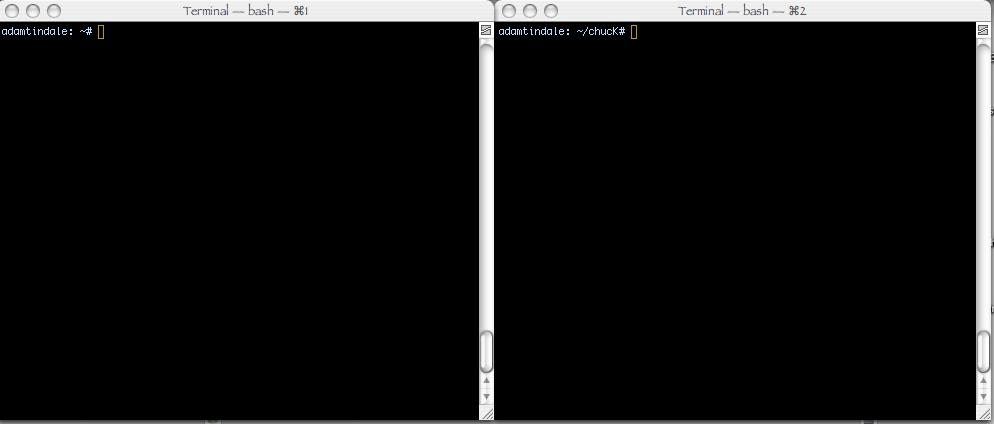
\includegraphics[width=\textwidth]{images/2term}

Here is what you do: open another terminal window just like this one. In this new window type:
\chuckterm{\prompt chuck \doubledash loop}

This will start ChucK running. ChucK is now waiting for something to do. Go back to your original window where you are in your ChucK home. Be careful. If you type chuck test1.ck you will start a second ChucK running test1.ck. What we want to do is add a script to the ChucK that we set running in our second window. We will use the + operator to add a script to our ChucK and the - operator to remove a script. 

\chuckterm{\prompt chuck + test1.ck\\
  \prompt chuck - 1\\
  \prompt chuck test.ck\\
  \prompt chuck test.ck\\
  \prompt chuck test.ck
}

What hapenned? That is the power. We added test1.ck. It was added as the first shred in our ChucK. Since we knew it was shred 1 we removed it by typing chuck - 1. Great. Next we added three copies of the same script! Isn't that cool? You can also do this chuck + test1.ck test1.ck test1.ck How do you keep track of shreds? 

You can ask ChucK how he is doing by typing chuck \doubledash status The shortcut is chuck \^ ChucK will answer in the other window where we left him running. He will tell you what shreds there are and what their id numbers are. He will also tell you how long he has been running. 

When you have had enough of ChucK you can go to the other window and use your fancy CTRL-C trick or you can type chuck \doubledash kill in your original window.   

\chuckterm{\prompt chuck \doubledash kill}

\section*{One Window ChucK}

So you think you are pretty good? One window ChucK is only for the hardest of hardcore. You have been warned. 

The concept is pretty similar to two window ChucK: first, you start a ChucK going, then you manage the adding and removal of scripts to it. How do you start a ChucK and get the command prompt to return, you ask? In your shell you can add an ampersand (\& ) after the command and that will tell the shell to run the command as a background process and give you the prompt back. 

\chuckterm{\prompt chuck \doubledash loop \& }

The rest is as it should be. You will have to be careful when writing your patches to not put too many print statements. When you print you will temporarily lose control of the prompt as the shell prints. This can be bad when are you are printing MIDI input. The same applies when you use the \doubledash status command to ChucK. It can also be fun to fight for your command line. Who will win?
